\documentclass[12pt]{article}
\usepackage{fancyhdr}
\usepackage{hyperref}
\usepackage[top=1in, bottom=1in, left=1in, right=1in]{geometry}
\usepackage{graphicx}
\usepackage{lastpage}
\usepackage{listings}
\usepackage{epstopdf}
\usepackage{indentfirst}

\begin{document}

% set up header and footer
\pagestyle{fancy}
\fancyhf{}
\setlength{\headheight}{1.25em}
\lhead{Mini-Project 2: Memory Allocation}
\rhead{CS 4410: Operating Systems}
\cfoot{\thepage\ of \pageref{LastPage}}

\fancypagestyle{first}
{
    \fancyhf{}
    \cfoot{\thepage\ of \pageref{LastPage}}
}

\lstset{language=C}

\title{Mini-Project 2: Memory Allocation}
\author{CS 4410: Operating Systems}
\date{Spring 2016}
\maketitle
\thispagestyle{first}

\section{Introduction}

For MP2, you will implement an interface that mimics dynamic memory allocation. Throughout this assignment, you will design your own data structure, implement the given function headers, and use pointer arithmetic to manage memory.

Along with a Makefile, you will be given two files: \texttt{alloc.c} and \texttt{alloc.h}. You are required to implement all of the functions specified in \texttt{alloc.c}, and you may not change the given function signatures. You are free to add any data structures or helper functions to \texttt{alloc.c} that you feel would be helpful. The documentation of the functions are found in \texttt{alloc.h}. \textbf{Do not change alloc.h.} When we grade your assignment, we will copy your \texttt{alloc.c} into a directory containing the original versions of \texttt{alloc.h} and the Makefile. Only your copy of \texttt{alloc.c} will be graded. Changing \texttt{alloc.h} in a meaningful way will likely result in your code not compiling when we test it. 

\section{Description}

Your dynamic memory allocator will consist of the following four functions, which are declared in \texttt{alloc.h} and will be defined (by you) in
\texttt{alloc.c}:

You may notice a common argument in the given function headers: \texttt{void *memarea}. In this assignment, you do not need to worry about getting a chunk of memory from somewhere. Instead, \texttt{memarea} will point to the total ``memory area'' that you will be managing. When it comes time for you to test your code, the test cases we provide will show you a few ways in which this \texttt{memarea} can be created. Do not assume that the \texttt{memarea} pointer is 8-byte aligned.

\begin{itemize}

\item \texttt{int alloc\_init(void * memarea, int size)} 

Sets up a new ``memory allocation area'' beginning at location \texttt{memarea} and of size \texttt{size} (in bytes). Returns 0 on success, nonzero if setup failed. Failure should occur if the size given is not large enough to hold your minimial memory administration (as you have designed it). This function should be called once before there are any calls to \texttt{alloc\_get},  \texttt{alloc\_release}, or  \texttt{alloc\_resize}. 

Your \texttt{alloc\_init} function should not create any structs outside of its \texttt{memarea}. Your implementation should support multiple \texttt{memarea} pointers which point to chunks of different sizes. This should happen naturally if you keep all of your metadata inside your \texttt{memarea} region.

\item \texttt{void * alloc\_get(void * memarea, int size)}

Allocates a block of memory of the given size from the memory area. Returns a pointer to the block of memory on success; returns 0 if the allocator cannot satisfy the request. Keep in mind that blocks of memory can be of size 0. The block address (which is returned to the user by this function) should be aligned at multiples of 8 bytes. This function is allowed to allocate \emph{more} than the requested size, but never less. The memory ``allocated'' by this function does not need to be zeroed out.

\item \texttt{void alloc\_release(void * memarea, void * mem)}

Releases the block of previously allocated memory pointed to by mem. If mem == 0, the function should do nothing. Released memory should be able to be allocated again by subsequent calls to \texttt{alloc\_get}. The memory released by this function does not need to be zeroed out.

\item \texttt{void * alloc\_resize(void * memarea, void * mem, int size)}

Changes the size of the memory block pointed to by mem, returning a pointer to the new block, or 0 if the request cannot be satisfied. The contents of the block should be preserved. If the location of the block changes, you can copy the contents by using \texttt{memcpy} or cast \texttt{mem} to a char* and copy the contents byte by byte. Keep in mind that the new block size might be smaller than the size of the allocated block that \texttt{mem} points to. As it was for \texttt{alloc\_get}, the return value should be 8-byte aligned. If mem == 0, function should behave like \texttt{alloc\_get}.

\end{itemize}

\section{Approach}

So, how do we organize this memory, keeping track of which parts of the memarea have been allocated/freed and also ensure we can re-use any memory that has been freed? You will need some way to keep track of each block of memory that is currently allocated. A common way of doing this is to place a ``header'' in front of each block of allocated memory with important information about that memory block. 

A primitive implementation of such a data structure could be as follows:

\begin{verbatim}
   struct m_header {
       unsigned int size;
   };
\end{verbatim}

Your memory area would then resemble a sequence of alternating headers and blocks as shown in Figure \ref{fig:memorystructure}. Ultimately, you will need something a bit more sophisticated than this, but this is a good place to start.

When you implement your dynamic memory allocator, think about the pros and cons of some common allocation strategies. A \textbf{first-fit} approach always gives the user the first memory block in the region that is big enough to fulfill the request. This provides the fastest response time, but is not necessarily the most space-efficient use of your memory region. A \textbf{best-fit} approach gives the user the \emph{smallest} memory block that fulfills the request. The allocator will not be as quick because it might search the entire list to find this smallest block, but this is a more efficient use of space. You might be able to speed up this search by maintaining pointers to free memory blocks of certain sizes. You will have to decide whether these efficiency techniques are worth the space overhead that they require. 

Another concept you will need to think about is \textbf{fragmentation}. After responding to many calls to \texttt{alloc\_get} and \texttt{alloc\_release} the memory region pointed to by \texttt{memarea} could become chopped up into small interwoven blocks of allocated and freed memory. When your memory region becomes fragmented, the \emph{sum} of the free blocks of memory might satisfy an \texttt{alloc\_get} request, but since they are not contiguous, the request will fail. Whether you implement a \textbf{first-fit} or  \textbf{best-fit} allocation strategy is just one way in which you control the fragmentation of your memory region. You should also think about how your implementations of \texttt{alloc\_release} and  \texttt{alloc\_resize} play a role in your ability to avoid fragmentation and satisfy future allocation requests. 

\begin{figure}
\centering
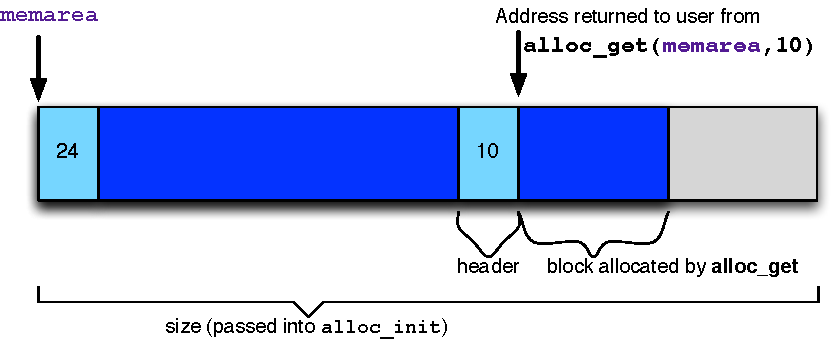
\includegraphics[width=0.7\linewidth]{simpleHeaderMP2}
\caption[Figure: Illustration of memory structure]{Example of a possible layout of \texttt{memarea}. Assume that a block of size 24 has already been allocated by the user. The Figure illustrates what memory looks like after the user calls \texttt{alloc\_get(memarea, 10)}. The light blue sections represent the headers, and the dark blue sections are blocks of memory which the user requested by calling  \texttt{alloc\_get}. 8-byte alignment is \emph{not} depicted in this Figure since the address of \texttt{memarea} has not been specified. Free memory is colored with gray.}
\label{fig:memorystructure}
\end{figure}

\section{Pointer Arithmetic}

To implement this assignment, you will want to use pointer arithmetic. As a basic example, see the following snippet of code:

\begin{verbatim}
   struct m_header *mh = memarea;
   return (void*) (mh + 1);
\end{verbatim}

As the type of \texttt{mh} is \texttt{struct m\_header*}, adding 1 returns a pointer that is \texttt{sizeof(struct m\_header)} bytes past the pointer \texttt{mh}. You should become familiar with pointer arithmetic if you are not already.

\section{Testing}
We have provided a few simple test files to show you how these functions might be called and used by an application. They might find very large bugs in your implementation, but these tests \emph{are in no way exhaustive} (or even particularly thorough). You \emph{must} create additional tests for your code to convince yourself that your code is correct. Try to come up with a number of cases that really stress your allocation functions. It's a good idea to test corner cases as well. For example, create a test that uses two different \texttt{memarea} pointers to two different chunks of memory. We will not grade your test cases, but if you do not write any, the chances that your code will pass our suite of tests is extremely small.

Also, you may find \texttt{gdb}, the GNU debugger, helpful while completing this assignment. (Tutorials can be found on \url{http://www.unknownroad.com/rtfm/gdbtut/gdbtoc.html})


\section{Clarifications/Tips}
\begin{itemize}
\item Your implementation does not have to be thread safe.
\item You should not call \texttt{malloc} anywhere throughout \texttt{alloc.c}. 
\item \texttt{uintptr\_t} in \texttt{<stdint.h>} is guaranteed to contain the size of pointer on the machine where the executable is running. You may find this useful.
\end{itemize}


\section{Evaluation}
Your implementation will primarily be graded on its correctness. It should be able to allocate memory of a given size, if there exists sufficient \textit{contiguous} memory in \texttt{void *memarea} to accommodate the request. If your code is extremely inefficient, our tests might time-out and you will then have points deducted for performance as well. (In practice, however, we have found that code which times out is usually incorrect and not merely slow.)

\end{document}
